%!TEX TS-program = xelatex
%!TEX options = -aux-directory=Debug -shell-escape -file-line-error -interaction=nonstopmode -halt-on-error -synctex=1 "%DOC%"
\documentclass{article}
\input{LaTeX-Submodule/template.tex}

% Additional packages & macros

% Header and footer
\newcommand{\unitName}{Embedded Systems}
\newcommand{\unitTime}{Semester 1, 2025}
\newcommand{\unitCoordinator}{Dr Chris Lehnert}
\newcommand{\documentAuthors}{Tarang Janawalkar}

\fancyhead[L]{\unitName}
\fancyhead[R]{\leftmark}
\fancyfoot[C]{\thepage}

% Copyright
\usepackage[
    type={CC},
    modifier={by-nc-sa},
    version={4.0},
    imagewidth={5em},
    hyphenation={raggedright}
]{doclicense}

\date{}

\begin{document}
%
\begin{titlepage}
    \vspace*{\fill}
    \begin{center}
        \LARGE{\textbf{\unitName}} \\[0.1in]
        \normalsize{\unitTime} \\[0.2in]
        \normalsize\textit{\unitCoordinator} \\[0.2in]
        \documentAuthors
    \end{center}
    \vspace*{\fill}
    \doclicenseThis
    \thispagestyle{empty}
\end{titlepage}
\newpage
%
\tableofcontents
\newpage
%
\section{Introduction}
\subsection{Definition of an Embedded System}
An embedded system is a combination of computer hardware and software
designed for a specific function or functions within a larger system.
These systems typically contain computer hardware \textit{within} their
implementation and are used in devices to simplify system design and
provide flexibility. Often, the user is unaware that a processor is
present in the device as an embedded system comprises a suite of
different components that communicate with each other to perform a
specific task. These components include the processor, memory, and
analog/digital ports---which form the microcontroller---and ports that
are connected to various input/output devices such as sensors,
actuators, and user interfaces---each of which interact with the
environment. This is illustrated in the figure below, where the grey
box represents the embedded system.
\begin{figure}[H]
    \centering
    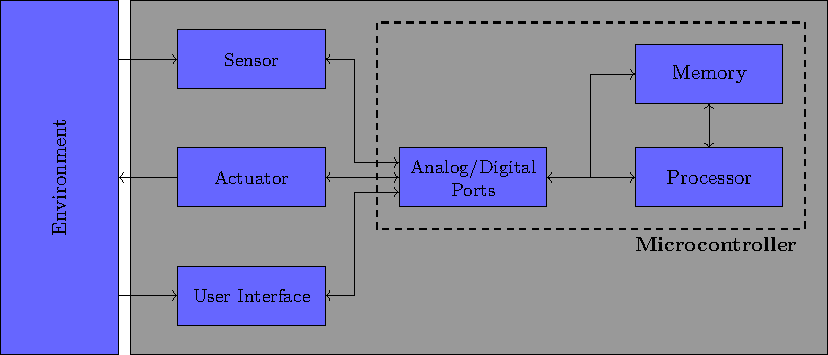
\includegraphics[width = \linewidth]{figures/embedded_system_structure.pdf}
    % \caption{} % \label{}
\end{figure}
\subsubsection{Types of Embedded Systems}
Embedded systems can be classified into three main categories:
\begin{itemize}
    \item \textbf{Centralised:} One node performs all work.
    \item \textbf{Distributed:} Nodes distribute work across sub-nodes.
    \item \textbf{Decentralised:} Nodes are only connected to peers in a network.
\end{itemize}
\subsection{Advanced RISC Machines}
Advanced RISC Machine (ARM) is a family of Instruction Set
Architectures (ISAs) for computer processors. These ISAs are developed
and designed by Arm Holdings so that they can be licensed to other
companies that design their own ARM-based processors. ARM processors
are found in many battery operated devices such as mobile phones,
tablets, embedded systems, and some newer laptops.

Reduced Instruction Set Computer (RISC) processors are popular in such
applications due to their high performance per watt and ability to
execute all instructions in a single cycle. Additionally, because the
architecture uses fixed-length instructions, instructions are also
easier to pipeline, leading to increased parallelism. The RISC
architecture focuses on small and highly-optimised instructions rather
than the highly-specialised set of instructions found on Complex
Instruction Set Computer (CISC) architectures such as x86. Although
this may seem restrictive, this allows instructions to be executed at a
greater frequency resulting in improved performance. Complex operations
can then be performed in software using these instructions.
\subsection{Characteristics of an Embedded System}
Embedded systems are characterised by several features. At a high
level, they may be designed to be:
\begin{itemize}
    \item Highly stable
    \item Time specific
    \item Task specific
    \item Cost effective
    \item Minimal in interface
    \item Easy to operate
    \item Real-time
    \item High-efficiency
    \item Reliable
    \item Memory constrained
    \item Power constrained
    \item Fault tolerant
\end{itemize}
\subsubsection{Design Goals}
These characteristics lead to several design goals in embedded systems
such as:
\begin{itemize}
    \item Reliability: Some systems may be critical to a mission, or
          life-threatening, and must be able to operate 24/7 without
          rebooting.
    \item Performance: Systems may need to respond to many events
          within a time frame using resources such as computing speed
          and power effectively. Constraints may need to be placed on
          inputs to prevent buffer overflows, and inaccuracies from
          floating-point calculations must be properly handled.
    \item Cost: Systems may be marketed to consumers and must therefore
          manufacturing minimise cost and be easy to produce.
\end{itemize}
\subsection{Real-Time Applications}
A system is said to be real-time if the total correctness of an
operation not only depends on its logical correctness, but also upon
the time in which it is performed. A primary design goal of real-time
systems is \textbf{meeting deadlines}.
\begin{itemize}
    \item \textbf{Soft real-time systems} execute as fast as possible requiring
          on explicit deadline on the response time.
    \item \textbf{Hard real-time systems} impose a strict deadline on the
          response time. If the deadline is missed, the system fails.
\end{itemize}
\subsubsection{Real-Time Operating Systems}
Embedded systems are typically developed using low-level programming
languages such as C, C++, and assembly, for their performance and
reliable compilation. The compilation process is different from that of
a desktop application where code is compiled into an executable file
which can be executed by the operating system. Instead, embedded
systems (or those with sufficient resources) make use of
\textbf{real-time kernel} libraries alongside application code to
produce a single binary image that is flashed onto the device. These
systems are known as real-time operating systems (RTOS). The kernel is
software that manages this real-time system by providing abstractions
for creating threads (tasks), scheduling, input/output operations,
memory management, and other functions in an operating system.
\subsection{Tiva C Series Microcontrollers}
This unit uses the Texas Instruments Tiva C series TM4C1294NCPDT
microcontroller which is housed on the EK-TM4C1294XL evaluation board.
This microcontroller chip is based on an ARM Cortex-M4 core and
includes several on-chip peripherals such as an Ethernet controller,
USB interface, analog-to-digital converters (ADCs), and timers. The
evaluation board also provides additional hardware such as LEDs,
switches, a touch screen, and other input/output devices, all of which
can be interfaced with the microcontroller.
\end{document}
